\chapter{中国未来怎么走?}
\label{chap:future}

笔者认为马克思足够深刻地揭示了现代世界的破坏性,但在建设性上乏善可陈,宏观或
曰大师叙事40余年来也欠缺实质性发展。笔者自然也更加无力去探讨中国未来发展路径
应是怎样,但自认可发现个别“忧国忧民”“专家”政策提案所描述未来美妙画卷背后隐藏
的真实破坏性——一些可以让党和国家陷入大崩溃泥沼、让人民生活日益困苦的破坏性。
笔者确信这个别“专家”要么是天真幼稚的蠢,要么是为背后利益集团服务的刻意为
恶。

当代世界的批判武器虽然在宏观和建设性上缺失,但历经200多年积累,其数量已积累不
少,可称是批判武器军火库了。边沁利己资本主义的侵蚀,人民批判意识日益增长,信
息化传播越来越便捷,使我们的一些“专家”话术也随之更加高明,可以十句话九句真,
隐蔽性极强。其中九句真话,主要立足批判现实存在的问题、弊端,也常常以人民的名
义批判政府,悲天悯人真是我见犹怜,比如减少城乡二元对立——户籍改革,劳动力自
由流动;加大民生支出、社会保障、居者有其屋。但剩下的那一句假话,才是其话
术“\textbf{精华}”所在,\textbf{前面九句真话、正确的话只是说明自己的正义和“洞见”,为其
  谎话打造合法合理性。真正要做的是悄悄引导党和国家、人民成为其背后利益集团待
  宰的羔羊。}

伪道学家、欺世盗名、祸国殃民、宵小鼠辈式的“专家”真不算少,道行更高者甚至可
以十句话十句真,比如可以流涕于中国财富分化之严重,摇旗呐喊中国要建立健全对富
人的累进直接税征收,呼吁国家招纳这类方向的专家进入智囊团,他自己其实却在国际
金融寡头公司从事着“资本管理”类的业务……真是让人叹为观止!高手啊!“高级知
识分子”啊!

笔者曾经真的失望于中国脊梁式的专家为何如此罕见,后来在写作本书、搜集资料的过
程中发现自己可能想错了。中国脊梁一样的专家不是凤毛麟角,只是他们大多乏名少利,
影响力有限,很少能站在光鲜亮丽的舞台前……不过当前世界已经应验了习总书记所
说“\textbf{百年未有之大变局}”,脊梁们还是能发声的多发一些,能做事的多做一些,晚一
些隐退于浊世吧……

本节一是说明世界各主要经济体在“百年未有大变局”中的共性背景,二是以《大国大
城》为例,对其批判,希望读者能够多些批判性思维,勇敢独立思考,谨防新自由主义
实践对公民权利的损害。三是建议党和政府对政策提案要进行不可行性研究,并提供部
分考量标准。四是谨防影子政府,与之战斗。


\section{背景:资本主义民主国家危机的共性}



沃夫冈·斯特里克在《资本主义将如何终结》\cite{JJDK201504024}\cite{streeck2017will}
一书中认为资本主义民主国家面临着同质的危机,尤其是美国,摘抄如下:

\improve[inline]{此书引用内容可进一步提炼总结,也可参考豆瓣宫野志保对本书的评
  论。 }
\begin{quotation}
  20 世纪 70 年代的\textbf{全球通胀}之后,发生了 80 年代\textbf{公共债务的上升},而 90 年
  代财政的巩固伴随着这一时期\textbf{私人债务的迅速增加},危机最终在2008年的金融危机
  中爆发,这种紧张局势被一个\textbf{不可持续的“向未来借款”}的过程所取代……40 年
  来,\textbf{失衡}几乎是各“发达”工业国和“发达”工业世界的常态。实际上,随着时间
  的流逝,人们已经不再把危机看成是纯粹的经济危机。这引发人们重新发现资本主义
  社会从前的概念——\textbf{资本主义是一种从根本上依靠私有资本积累连续过程的社会秩
    序和生活方式。}

  日益去工业化的资本主义国家轨迹的三个长期趋势。\textbf{首先是经济增长率持续下降},最
  近因2008年的事件而加剧了这一趋势;\textbf{二是主要资本主义国家整体负债程度普
    遍而持续的上升},40 年来,这些国家的政府、家庭、金融以及非金融企业不断累
  积起大量债务;\textbf{三是几十年来,伴随着债务增加和经济增长下降,收入与财富分配
    的不平等均处在上升过程中。}

  多年来,这三者似乎已经相辅相成:低增长加剧了分配冲突,加剧了不平等;不平等通
  过限制有效需求来抑制增长;高额的现有债务堵塞了信贷市场,增加了金融危机的可能
  性;过度增长的金融部门既是经济不平等的结果,也是经济不平等的加剧,等等。

  现在很清楚,资本主义世界的民主国家不是一个主权国家,而是\textbf{两个主权国家:下
    层的人民和上层的国际“市场”。}全球化、金融化和欧洲一体化削弱了前者,加强
  了后者。现在,权力的平衡正迅速向高层转移。\textbf{以前,领导人需要了解和使用人民
    语言;今天,他们必须掌握国际“市场”这一金钱语言。“人民耳语者”由“资本
    耳语者”接替。资本期望领导人知晓可保障投资者以复利收回资金的秘密戏法。}

  \textbf{资本主义可以由于过于成功而破坏其自身。}我所想像的资本主义终结,是资本主义
  由于其自身的原因而慢性衰败的过程。虽然我们\textbf{无从准确知道}资本主义什么时候消
  失、如何消失、以及替代资本主义的将是什么制度,\textbf{但重要的是,目前没有力量能
    够扭转经济增长、社会平等和金融稳定的恶化趋势并终结三者之间的相互强化}。

  当今经济和社会混乱背后存在着\textbf{结构性紧张和矛盾,社会科学几乎无能为力帮助解
    决这一问题。然而,它所能做的是揭示它们,并指出其历史连续性,以便充分理解
    当前危机。}它可以,并且必须指出\textbf{民主国家正在戏剧性沦为全球投资者寡头集团
    的债务催收机构}……今天,经济权力似乎比以往任何时候都更加成为政治权
  力\footnote{笔者注:新自由主义所要求的是经济自由优于政治自由。笔者妄论,可以认为新
    自由主义要求经济权力大于政治权力,政治权力沦为经济权力附庸。},而公民似乎
  已被完全剥夺了自身捍卫民主的力量,以及向政治经济施加影响的能力;公民的利益
  及其诉求与资本所有者的无法相提并论。

  事实上,回顾1970年代以来的一系列资本主义危机,仿佛真的有可能在发达资本主义
  中找到一种新的(即使是暂时的)社会冲突解决方案,这一次完全有利于现在牢固地扎
  根于其政治上无懈可击的据点——\textbf{国际金融资产阶级}。\todo[inline]{笔者对“事
    实上……”这句话的理解和翻译有问题,希望读者能提供中译版原文或者更好翻译。}

  % 只有扭转社会分裂持续加深这一趋势——资本主义在20世纪末和21世纪初的标
  % 志——才有可能使现代社会摆脱以无节制地生产有毒资产来设计合成增长来确保国
  % 内和平的强迫。
\end{quotation}

\section{大国大城=超级资本原始积累}

\subsection{大国大城概述}

陆铭教授写了《大国大城》,概括来说,他希望“在集聚中走向平衡”,政府发力发展
节约空间和时间的\textbf{大城市规模集约经济}——户籍改革,劳动力自由流动;大城市不怕
大、不怕扩建,敞开发展并吸纳劳动力,实现人员高度集聚的规模经济。

他认为,“拥挤Time、污染Grime和犯罪Crime问题这三种“城市病”对于中国来说并不
可怕,事实上可能并不严重。大城市在合适政府政策下也不会陷入贫民窟拉美化,且更
应去实现高密度基建。

过往土地金融导致地方以邻为壑、各自为政,重复建设、高大全项目体系可以休矣。当
然,这点批判完全没问题,许多专家也痛陈这一弊端,本书也涉及,这已是一种定
论。但关键是,要做什么!

\subsection{具体批判}

笔者无意于多么科学详实、引经据典地说明自己的批判观点,对于这样错漏百出、昭然
若揭的书来说并无必要。

接下来笔者逐条引用《大国大城》陆铭观点,然后进行具体批判:

\begin{enumerate}

\item 无知之幕

  \begin{quotation}
    美国的政治学家罗尔斯在他的《正义论》当中提出,一个问题中所涉及的所有各方,
    都应该被放在同一个标杆之后,在那儿\textbf{没有角色之分,也没有社会差异},这样的
    原则被称为“\textbf{无知之幕}”(veil of ignorance)。更通俗地说,其实这就是国
    际版的“换位思考”和“己所不欲,勿施于人”,这意味着在公共政策的讨论当
    中,\textbf{每一个公民所持的观点应该与自己的社会身份无关。}再换句话说,\textbf{公民所
      持的观点不应该跟自己是否在当前处于既得利益的位置有关。}


    中国的地方政府最大化本地利益,缺乏彼此之间的协调,国家利益被忽视,这极大
    地影响了中国发展的道路和可持续性。\textbf{中国已经到了呼吁每一个省、每一个市、
      每一个县、每一个人放弃本地思维,顾全公共利益的时候了。}(中央的更加集权,
    行政性配置,是否可能?地方不均衡如何解决?落后地区如何照顾?)


    不管是通过\textbf{财政转移支付}的方式,还是通过\textbf{帮欠发达地区还债}的方式,\textbf{发
      达地区都需要负起相应的责任}。读者可能会问,发达地区为什么要负起这个责任?
    道理并不复杂,因为这是\textbf{统一国家的必需},而且,发达地区恰恰是因为处于一个
    统一国家和统一货币区的内部,享受了统一市场的好处,获得了来自欠发达地区不
    断流入的劳动力资源,并且恰恰因为自身是这个国家统一货币区的一部分而成了金
    融中心。\textbf{只想要统一的好处,不想承担统一的义务,这是任何国家的政治都不会
      允许的。}
  \end{quotation}

  “无知之幕”之正义本身没有错,但当前世界不正是笼罩在功利利己这一经济学倡导
  的“理性”之下么?陆教授知道“\textbf{发达国家才不会以天下大同为己任呢!}”但似乎
  不知道自由经济学家们口中所说的\textbf{利己“理性人”,不止包括人,也实际包括着各级
  各处人的组织。}从何让各级各处组织和个人放弃自利,去实现这无知之幕呢?中央如
  何呼吁和管控?级级以邻为壑,事权层层下压,财权层层上收的过去,振臂一呼就变
  成大同天下,统一大国了?真好!共产主义一夜间到来了!真是正确又毫无营养的梦
  话。


  我们回到恩格斯《论住宅问题》,看到了历史的轮回:
  \begin{quotation}
    \textbf{现代的国家不能够也不愿意消除住房灾难。}国家无非是有产阶级即土地所有者和
    资本家用来反对被剥削阶级即农民和工人的有组织的总权力。\textbf{个别资本家}\footnote{恩
      格斯注:这里与问题有关的只是资本家,因为\textbf{参加这种事业的土地所有者首先
        也是以资本家资格出现的}}\textbf{不愿意做的事情,他们的国家也不愿意做。}因此,
    如果说个别资本家对住房短缺虽然也感到遗憾,却未必会受触动而去从表面上掩饰
    由此产生的极其可怕的后果,那么,\textbf{总资本家,即国家,也并不会做出更多的事
      情。国家顶多也只是会设法在各地均衡地推行已经成为通例的表面掩饰工作。我
      们看到的情形正是如此。}
  \end{quotation}


  % (“资本家不愿做的事,政府也不愿做”,为什么不让资本家去做呢?因为外部性?
  % 可实际上在历史经验及现实情况下,前者是政府的持续赤字,后者是太过乐观——政
  % 府的无能为力(包括美国))

  笔者知道,资本和性质等问题较为敏感。这里主要请读者理解。诚然,资本主义不完
  美,相当具有破坏性,但至今仍是革命性的和先进的,尚未有可以取代的生产关系。
  过去的所谓社会主义其主体其实仍是列宁所说国家垄断资本主义,社会主义或许并不
  具备充要科学成分。中国不能不走向这条道路,不然早就崩溃,只是我们走的太快,
  也舍弃了太多太多……本章首节引用了沃夫冈·斯特里克的几段话。在他看来,马克
  思可能悲观了,\textbf{资本主义如今日益严重的危机可能在尚未有新的革命性生产关系出
    来之前终结}。笔者对此抱有怀疑。

  至于国家,也请理解这番直言。笔者只是一介草民,于国于家无用,身无长物;没有
  加入什么结社团体;更无什么图谋不轨。只是世界各国如今都太危险了,中国作为各
  大国强国眼中的大肥肉,皆欲分我血肉、食肉寝皮,更是危险中的危险;而国外垄断
  金融寡头对我国的侵蚀程度并不乐观,国家肯定有相关了解,情况应当比大部分人想
  象的要更加可帕。笔者说出来,便想给出一个小压力,使国家不至于那么乐观,政策
  后果不至于那么坏,能减轻一些就好。

  \todo[inline]{以上部分太尖锐?删减?}

\item 用人均GDP、人均收入和生活质量来考量区域平衡

  \begin{quotation}
    应该从GDP总量增长的考核转变为\textbf{人均GDP的考核}。特别是对那些人口流出地来说,
    追求人均GDP、人均收入和生活质量才是长久之计,

    经济学家的研究发现,在欧洲,收入不平等减少快乐,而在美国,这种效应却不强。
    这实际上就和美国社会不同收入阶层之间的流动性更强有关,其实,\textbf{“美国梦”的
      道理就是说每个人都平等地拥有致富的机会}。
  \end{quotation}

  前文已述(见\cref{sec:gdp}),GDP、总收入的加总方式,无法说明分配不均、贫富
  差距、社会福利这类问题。大区域(比如美国的州)人均的本质仍是加总,同样无法
  说明这类问题。陆铭进而通过美国各州人均GDP比较平衡,证明美国区域发展均衡。美
  国梦“每个人都平等地拥有致富的机会”,哈哈哈哈……美国财富不平等可
  见\cref{tab:gini}。

  \begin{figure}[ht]
    \centering
    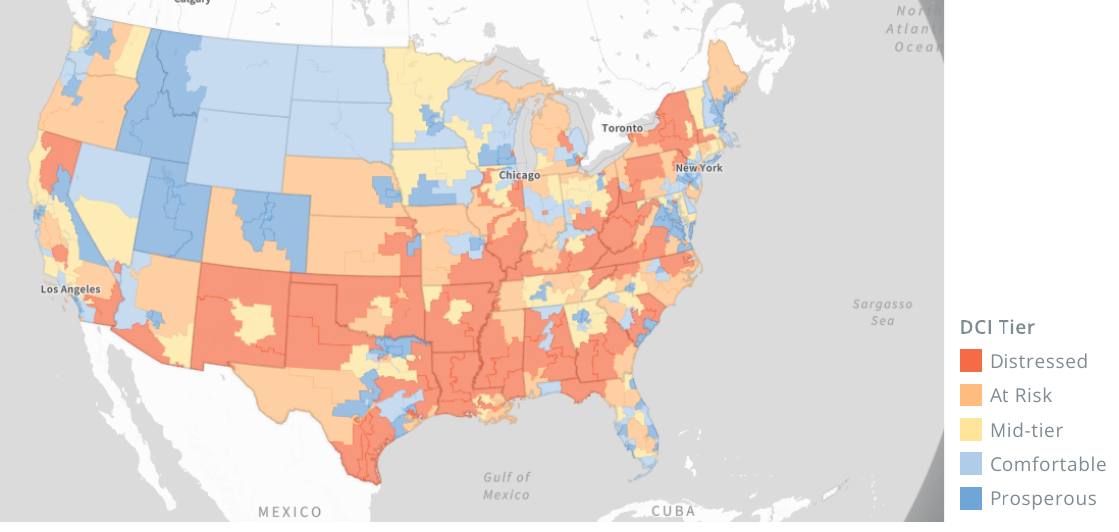
\includegraphics[width=0.9\textwidth]{figures/DCIbyDistricts.png}
    \caption{\label{fig:DCIbyD}美国困境社区指数(按districts划分)}
    \capsource{来源:\href{https://eig.org/distressed-communities/}{美国经济创
        新集团}}
  \end{figure}

  也可以参考美国经济创新集团(The Economic Innovation Group)发布的困境社区指
  数(DCI,the Distressed Communities Index,见\cref{fig:DCIbyD})。对困境社
  区指数DCI的中文介绍可见澎湃 《美国社区评价:困境社区指数和繁荣城区体系》。
  有兴趣的读者可以根据以上DCI链接网址,进一步了解美国区域不平衡。

  \begin{quotation}
    但是,城市化和地区之间的自由移民是一个\textbf{几十年甚至上百年的过程},在这个过程
    中,如果我们只看\textbf{特定时段的局部地区},就可能会觉得,劳动力流动并没有带来地区
    间收入水平差距的缩小。
  \end{quotation}
  陆铭倒是知道均衡需要长期(实际上根本不可能均衡)。可在几十年甚至上百年的区
  域失衡中,中国中央和地方、地方和地方、政府和人民的矛盾恐怕早已内爆了。

\item 不可能三角

  \begin{quotation}

    第一,国家的统一。

    第二,经济效率的提高。

    第三,区域之间的平衡发展。

    大国发展的“\textbf{不可能三角}”,而如果要破解这个“不可能三角”,就必须改
    变“平衡”的定义,将经济资源和人口均匀分布意义上的“平衡”,转变
    为\textbf{人均GDP、人均实际收入和生活质量意义上的“平衡”},而这种人均意义上的
    平衡恰恰是可以在人口自由流动的过程中实现的,不需要大规模地采取行政控制的
    手段来对人口流动进行限制。
  \end{quotation}

  前面一条已述当前人均“平衡”的荒谬。那么按陆铭说法,我们还是要面对不可能三
  角。我们是要国家的统一,还是经济效率的提高,还是区域之间的平衡发展呢?事实
  上会走到哪一步?

  恐怕这三角三边全部失败,只留资本寡头的胜利,他们可以资本外逃或当买办。

\item 持续发展

  \begin{quotation}
    未来中国的严峻挑战是城市部门是否能够\textbf{不断地提高劳动生产率},并且创造出越
    来越多的就业岗位,特别是\textbf{服务业岗位},从而吸纳更多的农村人口进城,使得城
    市化率不断提高,直至75\%,甚至80\%以上的水平。我们应该担心的,不是劳动力
    总量的枯竭,而是未来城市是否具有不断提高劳动生产率的能力。

    大家可能会怀疑,中国这样一个人口大国,能够实现75\%以上的城市化率吗?问这
    个问题,在本质上就是在问中国能不能\textbf{实现经济持续增长,最终成为发达国家}。
    未来中国的城市化率到底能够提高到什么程度,主要是看城市部门是不是能够\textbf{持续
    地提高生产率,并为农村进城的移民源源不断地创造就业,}如果能做到,农民就可
    以不断地减少,最终,通过农业的规模化经营提高\textbf{少量农民的收入}。
  \end{quotation}

  进城农民可从事餐饮、家政、网约车、快递、外卖等服务业,大城市伟大规模的服务
  业,能容纳那么多人呵!

  笔者认为,\textbf{当前世界环境及生产关系之下,从无“可持续发展}”。即使在主流经济学,也只有
  上升和下降的“\textbf{经济周期}”。可持续发展是梦,或是谎言!我们必然要经历下行期,
  甚至可能就在五年内、后年、明年。中国市场经济以来,没有经历过一个完整的经济周
  期,这使我们太乐观了,真的太乐观了……

  不可能持续发展的境况下,陆自己的论述就会将我们引到农民数量不可以不断减少,
  或者被迫挤进城市成为贫民。这点无需多说。

\item 政府支出和中央转移支付

  我们的陆教授说了几句冠冕堂皇的话,既好听又正确!但能做的是什么?做不到的后
  果又是什么呢?

  陆几处说到:
  \begin{quotation}
    \textbf{社会保障健全}则储蓄的动机将减弱。

    通过\textbf{中央向地方的财政转移支付,可以为人口流出地的养老提供更多资源。}更重
    要的是,\textbf{全国的养老保障体系将逐步走向一体化},这时,即使人口流出地面临更
    为严重的老龄化问题,也不需要担心了,这才是解决问题的根本出路。

    农民在放弃土地的时候要满足\textbf{自愿、有就业、有社会保障、土地(或建设用地指
      标)能够市场定价这几个基本的前提},让农民\textbf{避免被剥夺}。而以禁止市场交
    易的方式来保障农民,这是最为荒谬的逻辑,其结果恰恰是给不尊重土地产权的行
    政性剥夺找到了借口。

    在“蛋糕做大”的情况下,中央财政就更有能力来进行\textbf{区域间和城乡间的财政转移},
    但未来的财政转移应该更多地用于\textbf{城乡和区域间公共服务的均等化},比如说提高欠
    发达地区中小学教师和医护人员的待遇,相应地减少欠发达地区(特别是农村)政府
    的财政负担,以促进区域和城乡间在生活质量上的平衡,实
    现\textbf{“动人”和“动钱”的良性互动}。

    如果一个城市可以通过\textbf{基础设施和人力资本的投入},从而放大正外部性,会引导城
    市进一步向有效的更大规模城市发展;如果一个城市可以通过\textbf{技术进步和政府的管
      理措施}减少负外部性,也可以使这个城市更加有效地运转。

    对于部分国家出现的贫民窟现象,要作有针对性的分析。城市经济是否可以持续增
    长,从而为农村移民创造就业是非常重要的问题,一些拉美国家经济增长乏力,制
    约了低收入阶层提高收入的机会。而在印度这样经济增长较快的国家,城市经济高
    度偏向现代服务业和信息技术产业,为低技能者创造的就业机会有限。

    中国城市的土地是国有的,这在根本上可以允许\textbf{中国城市政府作出更好的规划},
    以及\textbf{向低收入居住区提供基本而必要的公共服务,来防止大面积贫民窟的出现。}
  \end{quotation}

  大国大城策略,要求在中国债务累累的情况下,国家继续进行巨额投资,发达城市要:
  巨资投入基础设施扩张。土地金融造就的大量衰退城市又被人为加大其人力流出,负
  债更加无力解决。中央要从自身和发达城市抽水,为衰退城市财政转移支付,用以发
  展落后地区的教育、培训、民生、公共服务等。你猜中央有多少钱?发达城市愿不愿
  意,会不会软性反抗,又能抽出多少水来?继续超发货币吗?

  普遍劳动力过剩、土地金融导致多数城市衰退的现状下,让农民挤入城市谋生,小城
  市市民挤入大城市,这一系列人造集约规模经济(资本史上也是一直如此人造,而非
  什么书上的自由市场。)之下劳动力只会更加溢出,失业后备军必然更大。政府需要
  在目前负债累累、养老保障覆盖面不足、养老金缺口巨大且持续扩大的今天,负担起
  更全面的社会保障。说得很好,点赞!资金从何而来?如何保障就业?危机之下农民
  又如何自愿放弃土地前往城市?农民、城市职工的社会保障肯定要政府支出,我们现
  实的社会保障什么水平,要达到这个目标又需要什么水平呢?不知从何而来的巨额支
  出!

  建设用地指标交易中,出卖土地指标方一般会是土地资源较大、发展落后的城市。农
  业工业化所需人力极少,即使地方政府获取了收入,也难免面临无法发展非农经济的
  困局。人力将会进一步流失,利得者是农业工业化的所有者,勉勉强强可加上地方政
  府。\improve[inline]{这点笔者不了解,或许错了,读者可以补充,但不影响本节结论。}

  正是大规模快速城市化造就大量贫民窟,城市化在消除过往贫民窟的时候,也将在未
  来产生条件更为恶劣的贫民窟。中国过去充满活力的“希望的贫民窟”——城中村因
  城市新增建设用地、发展工业和房地产中大部分消亡,但将在步步改造中产出生活条
  件恶劣、犯罪事件频发、公共服务无法保障、没有明天的“绝望的贫民
  窟”(见\cref{sec:hopedespair}),届时将处处有“深圳三和”,里面到处有不怀希望
  的“挂逼”。

  20年来,各行各业均有不少人担心中国出现“拉美化”,陆认为中国实现大国大城就
  不会“拉美化”,要求政府“作出更好规划……基本而必要的公共服务”等等。\textbf{其
    真实目的是将可能出现——其实是必然出现的——“拉美化”贫民窟的责任转嫁给
    政府!}不是我的政策提议不好,而是因为政府技术和管理水平差,超出预期!不知
  道读者们是否还记得本书提及的个别专家学者对80年代中后期双轨制的论述。
  政府管理水平又如何提高至可以应对其中种种问题?政府实际能力的限度是多少?我想政
  府和专家都应该明白。

  当前地方以邻为壑、各自为政,陆对此也批判。但陆所要求的是1980年代以来一个从
  未有过的空前集权的中央政府!一个具备超凡入圣管理水平的政府!一次\textbf{超级大跃
    进}呵!完全无视中央和地方关系的复杂化,更重要的是无视现实境况。

  土地的市场定价,呵呵,恐怕是软硬暴力下才会有这样一个“市场”吧。这条放在本
  节总结时再论述总结。


\item 地方比较优势

  一些“专家”提出了常人都不理解的“比较优势救国论”,倡议中国大力发展生态旅
  游农村、农家乐、山海旅游景点或港口均是如此,大多数人第一反映是这究竟能对这
  么大中国的经济帮助多少?类似观点有时并非是“专家”高瞻远瞩,\textbf{更可能是别有
    用心}。将特殊提升至一般后,建立自己提案的伪合法性和伪有效性,隐藏其真实动
  机。

  个别、特殊、一般(普遍)这三个基本的哲学概念及其矛盾和张力常常被忽视。国家
  和人民要小心对待任何“比较优势”的说法!比较优势基于区域\textbf{特殊性},一定要考察
  相应提案能覆盖和折射中国多少区域;有相近比较优势的区域过多也会使其同质化,
  走向\textbf{一般性},丧失\textbf{特殊性}。

\end{enumerate}

\subsection{总结——美国式道路的超级原始积累}


本节以陆铭《大国大城》为例展开批判,并非因为陆铭是段位很高的“高级知识分
子”或很专的“专家”。相比于他那些可以十句话里九句真、只有一谎为利益目的的同
路“专家”,他的话术并不高明,往往以片面论述全面,以个别论证一般,以小作文抒
情代替论证,但其“大国大城”政策提案却真是太可怕了。

大国大城其实并无多少新意,其实只是我国政府2012年所提“新型工业化、信息化、城
镇化、农业现代化(工业化)”新四化的扩大版,我们也一直在走这条道路。要说有新
意,那就是倡议立刻将区域限制由省市县直接扩展到国家一级。

\textbf{土地的自由留转、自由市场定价没有在过去200年出现过,也不会在未来几年实现,只
  能在农业税、政府和资本协作的羊吃人、农业工业化挤出小农生存空间等软硬暴力中
  实现。}希望是不学无术的笔者错了。

对马克思政治经济学有基本了解的人,便可以看出这是赤裸裸的超级“\textbf{资本原始积
累}”,并且是超级“\textbf{美国式道路}”。

我们回看历史,美国式道路是建立在殖民者造成的印第安人累累白骨至上。19世纪中后
期俄国民粹派知识分子正是害怕血淋淋原始积累才积极学习马克思,向马克思求助,探
索社会主义道路。1900年代之初政治强人如列宁认为俄国要生存和发展最好是经过“美
国式道路”——农业工业化资本家,也只敢借希望由沙皇俄国来推动。斯大林掌权后搞
了古拉格和大迁徙,效果并不是很好,并造成巨大灾难(
见\cref{subsec:shenkerenshi})。毛泽东尝试大兴农田水利基建消化农村剩余劳动力
的社会实验失败后,也只是城乡二元对立固化、工农剪刀差,先保障城市经济,同样不搞
或者不敢搞“美国式道路”。对于中国现状来说,这仍是极为可怕的、血淋淋的!

大量失地农民,过剩的产业后备军(失业和半失业者),无限压低的工资……中国人已
经不是饿不死就不乱的中国人了,届时党和国家将面临极大危机,甚至是前所未有的危
机!陆的真实目的到底是什么?谁最得利?最后的胜利者只有国内外的金融和土地食利
者——金融垄断资本家(土地已彻底归于金融。)。

这便是新自由主义,步步吸取国家政府和人民血液,至死也不休,定要寝骨食皮。矛盾
的对象最后可能直接被转嫁给党和国家。“啊,政策是好的,让和尚念歪了”!党和政
府不可不防啊!

事实上,笔者还见到有其他“专家”设此同样路径——他们一方面给糖衣炮弹、赞美党
和国家;另一方面将必然会失败的内容,同时也是私人资本不愿承担的内容,推给国家
负责。例如倡议政府和国有企业负责必然会被债务压垮的巨型重固定资本投资,同时要
求国家负责消除届时兴起的条件愈来愈差的贫民窟等。

我国在1992年后没有经历完整经济周期,1998、2008年左右依靠原垄断在国家的土地红
利超发货币渡过难关,但不会一直这样下去。除非我们能战胜美国资本,危机转嫁美国;
或者战争侵夺他国财产、灭失自己人口等等……这都是太过邪恶的道路,并且有着艰难
未知后果。

党和国家需要更悲观反思危机,需要更谨慎小心政策提案,甚至可能需要坦诚面对和释
放一些危机。超发货币不持续,其实谁都知道……

% 一方面,对于市场上的债务违约,中央当然希望打破“刚性兑付”的预期,以免将什
% 么责任都揽在中央,让人们形成地方债务没有风险的预期;另一方面,面对事实上已
% 经难以偿付的地方债务,最终还是会被认为将由中央政府来兜底,从长期来看,这也
% 恰恰可能造成地方政府不计后果地借债的局面,这就是经济学里典型的“道德风
% 险”问题


% 世界主要经济体基尼系数基本已达70以上,无论是国家人均还是大地区级的人均GDP这两
% 个指标已难以说明其中人民的经济水平,它们更能说明的只是富人资本。

% https://m.thepaper.cn/newsDetail_forward_22666274

% 吸纳不了,黄奇帆 美国 金融华尔街30万人





% 我并不是反对为欠发达地区提供财政补贴,我要讨论的是,在政府进行财政转移的时候,
% 应当考虑转移的数量、地点和结构,如果违反市场经济的规律,盲目追求人口和经济资
% 源的均匀分布,那么,一系列低效率的后果就必然会出现。

% 西部和边陲的发展,因为这是政治和国防的问题,但政治和国防与我们这里讨论的问题没什么关系。

% 2014--2020新型城镇化规划只是北京、上海超大城市限制发展。

% 在转型期,由于公共服务的享受权仍然与户籍身份挂钩,同时,在公共服务供给不可
% 能短期内快速增长的情况下,改革不能在一夜之间取消户籍与公共服务的挂钩,因此,
% 户籍的转换或者特大城市实施的积分落户制度就必须设置门槛,形成对于一部分人的
% 事实上的公共服务歧视。那么,这样过渡时期的“歧视”应该遵循什么原则?这就要
% 本着理性原则,尽量将仅仅为公共服务而流动的人口识别出来。

% 因此,政府可以通过一定的办法来识别出仅仅为了公共服务而迁移的人群。其中,最
% 好的办法就是认为有就业记录和社会保障记录的人群是以就业为主要目的的迁移人群。
% 虽然这一标准并不完美,却是现行条件下能找到的最好指标。





% 尊重的规律是什么?是有权势者对无权势的尽情盘剥。

% 社会保障健全则储蓄的动机将减弱。

% 经济学家的研究发现,在欧洲,收入不平等减少快乐,而在美国,这种效应却不强。
% 这实际上就和美国社会不同收入阶层之间的流动性更强有关,其实,“美国梦”的道
% 理就是说每个人都平等地拥有致富的机会。

% 中国城市的土地是国有的,这在根本上可以允许中国城市政府作出更好的规划,以及向低收入居住区提供基本而必要的公共服务,来防止大面积贫民窟的出现。

% 避免城市出现贫民窟问题的关键是要通过城市发展源源不断地为进城农民创造就业机
% 会,并且为其提供适度的公共服务和社会保障。

% 对于部分国家出现的贫民窟现象,要作有针对性的分析。城市经济是否可以持续增长,
% 从而为农村移民创造就业是非常重要的问题,一些拉美国家经济增长乏力,制约了低
% 收入阶层提高收入的机会。而在印度这样经济增长较快的国家,城市经济高度偏向现
% 代服务业和信息技术产业,为低技能者创造的就业机会有限。


\section{建立健全政策提案的不可行性报告}

前文已说太多,直入主题吧。笔者建议党和国家建立健全政策提案的不可行性报告,慎
重对待任何人对中国未来走向的提案。可包括如下内容:
\begin{enumerate}
\item 建立各种倾向专家、官僚组成的评审机制,建议倾向于有才,但少名少利或暂受抑制的人员。

\item 由情报机关牵头对提案人及其关联人员、组织做背景调查、政策倾向。

\item 提案人需说明其提案倾向于投资还是消费,二者内容如何划分,篇幅不必长,但必须
  涉及具体举措。

  如提倡“居者有其屋”的赵燕菁应说明政府需投资多少,债券是否会造成美国式次贷
  危机,城市报障房规模到底能多大、能容纳多少人,如何健全报障房租户审核,退出
  机制如何,报障房又如何不影响商业房等,与19世纪英国的住宅报障计划有何本质区
  别,而不是简而化之。

  对可能出现的破坏性后果必须详细说明。《大国大城》就是未对破坏后
  果详细说明的反面例子,前文已述。

\item 警惕一切需要政府大力兜底的政策。我们的一些提案者们已经习惯于拍政府马屁的同
  时,却让政府“负责”某些必然或极可能失败的内容。届时出了问题,“非我之罪,
  罪在政府,政府大罪!”。

\item 提案不可行性报告是领导接见提案人的前提。
\end{enumerate}
\todo[inline]{希望大家补充不可行性报告!}

\section{谨防影子政府}

美国有Shadow Government(影子政府),或曰Deep state(深层国家),现在基本上是
易得认识。笔者甚至怀疑New World Order(新世界秩序,多国顶层资本精英和政府权力
贵族组成的幕后世界政府)到底是阴谋论还是现实……

世界各主要经济国普遍持续超发货币,制造货币炸弹摧毁之前的货币;寅吃卯粮的丧失
理性,进行着“击鼓传花”和“只要我跑得比你快”的庞氏骗局金融游戏;为了躲
避1929年美国经济大萧条危机而持续吹大泡沫、给未来炸弹持续装填炸药;为“大到不
能倒”甚至“大到不能判刑”的金融资本造血输血;人民在超发货币中不停交着铸币暗
税……负债累累的政府并不是胜利者,暂时的胜利者只有财富分化日益严重下越来越富
的顶级富人阶层。当然,他们现在也面对天威难测的大变局。(
见\cite{piepenburg2022gold}、\cite{streeck2017will}、\ccref{sec:podestamail})

结合新自由主义批判说法,影子政府应是金融精英和权力贵族的合体,以政府透支于公共
债务减轻投资压力、加快资本流转,并做私人贷款的催债机构,来使自己的资本增殖。

读者们应该比较熟悉日本和韩国“\textbf{财阀}”一词,其实财阀即\textbf{康采恩垄断集团}。康
采恩以其金融垄断机构为核心或直接设为母公司,直接或间接控制多行业领域中的企业,
往往涉及各行业全链条或主要部分,实现横向纵向全面垄断,为金融中心服务,获取
超额利润。

中国也有自己的康采恩,如一些IT集团(这很可能也只是显露出的冰山一角
)。2020年7月15日,蚂蚁金融服务集团运营主体浙江蚂蚁小微金融服务集团股份有限公
司正式变更企业名称为蚂蚁科技集团股份有限公司。同年10月24日,马云在上海第三届
外滩峰会上发表一番惊世骇俗的演讲,笔者认为其深层目的在于欲让蚂蚁科技集团股份
有限公司这一“科技公司”取代央行货币的四大职能——价值尺度、流通、贮藏、支付
手段;还要超高杠杆、无节制发展金融信用;消泯国家金融监管职能乃至世界金融监管
体系!

传统的金融公司都受到巴塞尔协议的限制,可是蚂蚁科技通过将自己“包装”成科技公
司绕过了监管,并且依托其行业垄断地位,大数据红利等获得了传统金融公司无法得到
的超额利润。一旦蚂蚁科技集团出现金融风险而国家不得不出手救助,就意味着让全体
国民被动帮它分担和承受风险损失。


2021年4月10日,市场监管总局依法对阿里巴巴集团处以行政处罚,并处以182.28亿元人
民币。2021年7月7日,中国金融监管机构对蚂蚁集团及旗下机构处以71.23亿元罚款,并
关停其旗下的“相互宝”业务。两次巨额罚款之后,阿里股票大涨,资本市场认为蚂
蚁“\textbf{利空出尽}”,投资信心回升……在其演讲和事后处罚上,我们都可以直观感受到
金融垄断资本的强势地位和野蛮狂妄。


中国体量太大,营养太丰富,国外反动势力意图阴谋颠覆中国之心未曾停歇。在当今残
酷的世界政治竞技场中,一个伤痛的中国将被诸多国家、甚至本国买办——金融精英和
腐败权力贵族群拥而上,饕餮而食,渣骨不剩,万劫不复。不了解当前世界政治这一残
酷性,要么是幼稚无知,要么是包藏祸心,望大家明鉴,莫要让亲者痛、仇者快。我们
砥砺前行吧。

党和政府一定要深刻理解并运用好习总书记所说“人民监督”“自我革命”两种武器,
一定谨防影子政府的产生,或者与已经产生的影子政府开展艰苦卓绝斗争。影子政府总
的意图是相通的——侵蚀中国国力和民生,借此满足自己对资本增殖的无限贪欲。


\begin{quotation}
  主人说,“你这又可恶又懒惰的奴仆!你既然知道我在没有播种的地方也要收割,没
  有撒种的地方也要收获,就应该把钱存入钱庄,等我回来可以连本带利还给我。”

  “所以收回他的一千银币,给那个有一万银币的奴仆。因为凡有的,还要给他更多,
  让他丰富有余;凡没有的,连他仅有的,也要夺去。把这没用的奴仆扔进外面的黑暗
  里,他必在那里哀哭切齿。”

  \raggedleft
  —— \quad《圣经·马太福音》 \qquad
\end{quotation}


% 是否正在酝酿,甚至已经形成呢?如果有不能不防啊。我想习总书
% 记所说“群众监督”和“党的自我革命”真实用意也在此。

% 习总书记进行了大刀阔斧,老虎也打的反腐斗争,取得很大成效。但作为最高领导人,
% 又是孤寒甚至孤愤的。

% 自大萧条以来,政策制定者很少(如果有的话)面临像今天这样多的不确定性。其中一
% 个例子是,市场不仅期望财政整顿,而且同时期望未来经济增长的合理前景。两者如何
% 结合在一起尚不清楚。

%   这里用两句话来说明间接税和直接税:

%    1、间接税是穷人税,每个人税率一样,比如普通商品的增值税。

%    2、直接税是富人税,根据累进算法,富人交更多的税,比如个税和尚未开征的遗产税。

% 美国直接税的大头是中产阶级,而不是富人阶级。


% 政商旋转门

% 常驻的匪帮,依靠垄断,全民收税……赵燕菁核心

% 大一统和合法性,转移支付,全民的,自建国后开始的

% 精神和物质文化需要,已不再是……人为打压后果……

% 财富分化加剧已是共识,就分配尽量公平几乎都有论述,那其应当说明如何可以归于公众?需仔细论述,魑魅魍魉往往在此不得藏身。

% 种种天方夜谭式的救市方案。

% 警惕一切需要政府、企业(现在预警下=持续负债)大力兜底的政策。如这些政策制造出来的贫民窟、发达地区向落后地区的转移支付(如大国大城的叙述矛盾,一方面反对转移支付,一方面又提倡向没有享受公共投资好处的地方进行适度的财政转移。。当然,前者是全面的,后者是个别方向的,如“落后缺失”,但是这两种转移支付真的有本质区别么?“问题是,什么叫支持当地的发展?是把公共财政投向欠发达地区直接建开发区办厂,还是把钱投向欠发达地区建设基础设施和公共服务?直接把钱投向生产性的项目就必须最终接受市场竞争的考验,如果经济欠发达地区恰恰是在地形比较复杂、远离大的城市中心和交通干线的地方,那么很有可能生产成本和运输成本过高,从而大规模的生产性投资缺乏市场竞争力。对此,看看全国遍地开花的开发区,看看政府砸了多少钱,换来多少产出就知道了。偏离当地比较优势的投资不仅不会有效地帮助欠发达地区提高经济发展水平,而且可能使这些地方背上沉重的财政负担,对此,前文已强调多次。同时,如前所述,在缺乏发展工业比较优势的地方,硬要搞招商引资,地方政府官员也苦不堪言,结果招来的往往还是东部不要的污染和高能耗产业。” PS:也要考虑其中的正确性,如当地比较优势的投资。道路和机场的建设更为重要。 ,政府的财政转移支付主要是用于支持欠发达地区的公共事业,特别是教育和医疗事业,从而帮助欠发达地区的居民提高生活质量。发达地区的教育和医疗事业正是个烂账,看美国 图)。

% “公众基金”也是解决贫富差距问题的社会新实践。通常的做法主要有两种:一种就是在生产循环的前端,通过生产资料公有制(也就是“国有企业”)来实现均富的目标。另一种就是在生产循环的后端,通过高税收和转移支付,实现均富的目标。

% 后者根据不同标准每年按照面积和效果评价获得非建设用地补偿金。

% 改革后,村集体的“田底”可以是混合的产权组合,并可在资本市场上转让。不同集体的产权可以合并,也可以到市场上“招商”,寻找能够提供优质公共服务的运营商。


% 为什么重资产要由政府提供?为什么企业不愿投入重资产?不盈利!

% 一国债务与GDP之比在五年内涨幅超过30%的话,大概率会在随后的五年内爆发经济危机,美国次贷危机后的十年,可以说连续已有两个五年债务都增长了30%以上。所以,按现行美国举债速度和赤字增加速度如果不变的话,要不了几年,美国经济将被债务大山压倒。

% 税收制度日益累退的特征

% 黄奇帆

% 美国会采取什么经济措施来缓和平衡美国政府债务率过高的问题呢?从过去几十年历史经验看,大概率会采取三种措施。

% 第一种是美元贬值、通货膨胀。为了维护美元地位,维持债务融资来源,美国采取直接违约的可能性极小,但却不能排除美国政府以间接方式违约。这些方法包括美元贬值和通货膨胀。有三个历史性案例:一是1933年,美国因美元贬值,废除国债的黄金条款,国债购买者不能按原契约换取相应黄金;二是第二次世界大战后,美国采取通胀办法,每年通胀6%,五年总债务占GDP比例能减少20%左右,十年能降低40%左右;三是1971年美国单方面停止美元兑换黄金,致使布雷顿森林体系崩溃,继而确定了牙买加体系。总之,采用美元贬值和通货膨胀变相违约,早已是美国减债减赤的惯用手法。

% 第二种是通过加息缩表剪羊毛,以邻为壑转嫁危机。美国每一次加息周期往往会演化出某一领域或某一地区的经济危机、金融危机。20世纪80年代以来,美国有4轮加息周期,80年代加息的尽头是拉美债务危机;90年代加息的尽头是亚洲金融危机;2003年开始的加息周期尽头是全球金融危机。目前这轮加息周期从2015年12月开始,2015年、2016年、2017年各加息一次,2018年已经3次,预期全年加息4次。那么,这次加息的尽头是在什么地方、什么领域出现大级别的危机呢?由于加息,美元走强,近几个月继巴西里拉之后,南非兰特、印度卢比、印尼盾、俄罗斯卢布、阿根廷比索都在大幅贬值。因此,现在大家有种预感,近期的新兴市场货币贬值是否表示新一轮金融危机将表现在新兴市场?

% 第三种是以全球经济老大的实力改变游戏规则,大打贸易战意图获取超额利益弥补、化解债务困境。美国经济结构有很大问题,其GDP中85%来源于以金融为中心的服务业,制造业只占11%。美国巨额的贸易赤字根本就是自己的经济结构造成的,而不是别国造成的。怪罪于别国,完全是一种得了便宜还卖乖的行为。金融业属于精英产业,对劳动力吸纳能力非常差,比如美国金融中心华尔街总共才吸纳30万人就业。

% 总之,解决危机最不能容忍的办法有三种:一是不能为了掩盖矛盾、缓和矛盾而把现在的危机推向未来,导致未来更大的危机;二是不能用一个倾向掩盖另一个倾向,走极端,采取一种措施解决一个危机而引发另一个更为严重的危机;三是不能以邻为壑地把自己的问题转嫁给别人,利用自己的强国地位、货币信用为所欲为。

% 理性个人自利……政审、背调,尤其是利益关系的简要报告。公司可以,政府也可以,这没什么出格的,何况事关国运。


%%% Local Variables:
%%% mode: latex
%%% TeX-master: "../main"
%%% End:
